\documentclass[11pt,a4paper]{article}
\usepackage{lac2013}
\usepackage{graphicx}
%\usepackage{natbib}
\usepackage{url}
\sloppy
\newenvironment{contentsmall}{\small}

\title{Music for Programmers (MFP): A Dataflow Patching Language}

%see lac2012.sty for how to format multiple authors!
\author
{Bill GRIBBLE
\\ \texttt{grib@billgribble.com}
}

\begin{document}
\maketitle

\begin{abstract}
\begin{contentsmall}
MFP is a graphical dataflow patching language in the tradition of Max/MSP
and Pure Data.  It expands on its predecessors by integration of
higher-level language constructs from Python, including a variety of data
types and operations and the widespread use of the Python evaluator.  A new
lexical scoping system, a \emph{layers} approach to building logical code
blocks, and a UI optimized for keyboard control are also featured.
\end{contentsmall}
\end{abstract}

\keywords{
\begin{contentsmall}
Patching languages, Python, JACK, OSC, Pure Data 
\end{contentsmall}
}

\section{Introduction}

Graphical patching languages have a number of basic principles in common. A
``patch'' is a computer program specified by a diagram.  The patching
system acts as the development environment, compiler, and interpreter for
this program.  The diagram consists of processing elements and connections
between them in the form of \emph{patch cords} or virtual wires.  Typically
patches exist and operate in 3 domains: the graphical domain, which
includes the visual elements displayed in the patch and any interactive
controls such as buttons and sliders; the control or symbol domain, where
patch elements communicate by sending discrete messages; and the signal
domain, where communication is in blocks of audio data.

Possibly because the ``patching'' metaphor is so familiar to electronic 
musicians, there exist several patching languages for audio and music, both 
commercial and FLOSS.  Notable examples include Miller Puckette's languages
(Max/MSP \cite{Puck:Max}, jMax, and Pure Data \cite{Puck:PureData}),
Blechmann's Nova/SuperNova \cite{Blechmann:Nova}, and Ross Bencina's
AudioMulch \cite{Bencina:AudioMulch}. The notion of a visual graph of
processing nodes is also popular in other domains, notably scientific data
collection where National Instruments' LabView \cite{NI:LabView} has used
this metaphor since 1986. 

In the Linux audio world, Pure Data is probably the leading patching
system.  Its large library of built-in and third-party modules make it a
versatile toolbox for audio synthesis, performance control, interfacing
with experimental input and output devices, video creation, and video
interpretation.  The user and developer communities are full of
enthusiastic, helpful, and talented people.  In short, Pure Data is
awesome.

However, in my experience with Pure Data I have been frustrated at times
with the difficulty of simple operations with basic data types like strings
and lists.  I am more proficient as a programmer than as a musician, so
this kind of thing annoys me perhaps more than most PD users.  Often
third-party packages are required to perform what seem to be elementary
operations on data.  Interpreting literal data entered in message boxes, or
building non-numeric values, often requires trial-and-error and results in
solutions that are nonintuitive for the non-guru.  Resolving issues of
names and namespaces often involves what appear to be kludgy solutions (I'm
looking at you, \texttt{\$0}).

When I was faced with tackling a significant project in PD (a system to
analyze the dynamic behavior of a piece of external audio equipment), I
simply could not bring myself to do it.  I wanted a different tool, with
more support for general-purpose programming and a more familiar approach
to data.  This was the genesis of MFP.  

I began to explore starting from a few basic goals: 

\begin{itemize}
\item[]
Use Pure Data's graphical metaphor and idiom as a baseline, without
attempting to preserve compatibility 

\item[]
Expose Python wherever possible, and use plain Python data natively

\item[]
Rethink name resolution and scoping

\item[]
Implement a clean and simple GUI that assists in the construction 
of patches 

\item[]
Expand the range of system, file, and string operations, to make
general-purpose programming easier

\item[]
Integrate readily into a variety of audio production workflows as an
instrument, a forensic tool, or an audio swiss army knife
\end{itemize}

The work-in-progress result of this exploration is MFP.  MFP includes
elements familiar to high-level language programmers, with a standard
library and graphical presentation layer that will be familiar to users of
Max/MSP and Pure Data, though there are many differences large and small. 

My hope is that it will appeal to patching musicians while providing a
stronger foundation for analytical, scientific, and general-purpose
programming.  The popularity of tools like LabView in domains other 
than music shows that dataflow patching systems can be useful in a variety
of control and analysis tasks, given an appropriate infrastructure.  MFP
should be of interest to musicians, particularly those focused on the
symbolic domain (MIDI, OSC, and generative music applications) where Python
will provide significant leverage, but also to audio software developers,
plugin authors, and recording engineers who need to build custom tools to
interact with audio data.

\section{Architecture}

MFP is implemented in Python 2 \cite{Python:2.7}, with C extensions for
real-time DSP.  In order to mitigate Python's Global Interpreter Lock (GIL)
bottleneck \cite{Python:GIL}, processing for each of the three domains
(graphical, control, and signal) is performed in a separate process.  The
three processes (``nodes'') are coupled via the \texttt{multiprocessing}
facility present in Python 2.6 and later. 

A patch, as represented in the user interface for editing or control,
appears as a multi-layered diagram of visual elements such as boxes,
controls (sliders, buttons) and displays (indicators, meters, signal
graphs) connected by lines representing communication pathways.  Some
connections terminate in \emph{vias}, which represent invisible communications
between endpoints.  Each element in the display domain has a corresponding
unit or connection in the control domain, and may or may not have elements
in the signal domain. The use of layers, ``wired'' connections within a
layer, and vias between layers evoke a printed-circuit board metaphor, but
this is not rigorously followed. 

The ``hello, world'' example in Figure 1 demonstrates the basic properties
of an MFP patch in the simplest way.  The literal string ``hello, world!''
is contained in a \emph{message box}, which is an interactive element that
emits its contents when clicked.  The \texttt{print} object is a
\emph{processor} which prints its argument to the MFP log window.  

In this example we see the first differences from Pure Data: in PD, it is
not possible without some difficulty to print messages containing commas,
since strings are not one of the basic ``atom'' types that can be represented
in message boxes.  In MFP, the literal contents of the message box are
interpreted at creation time by the Python evaluator; a message box can
contain any Python expression, including literal data or code that
evaluates to a Python object.  In this case, if the message box was filled
with the text \texttt{", ".join(["hello", "world!"])}, which is an idiomatic
Python expression for joining a list of strings into a single
comma-separated string, it would have produced the same message to the log
when clicked: \texttt{"hello, world!"}

\begin{figure}
    \centering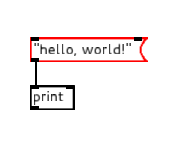
\includegraphics[width=2in]{hello_world.png}
    \caption{``Hello, world'' program in MFP (\texttt{doc/hello\_world.mfp})}
\end{figure}

\subsection{Layers}

Layers break a patch into ``pages'', providing visual grouping and
separation of elements, and are are somewhat equivalent to code blocks in
traditional languages or subpatches in Pure Data.  Layering is a key
mechanism for program decomposition in MFP.  

Figure 2 shows views of a more complex multi-layered patch and the
application context when using it.  This patch implements a basic looping
sampler inspired by the Akai Headrush looping pedal.  Four layers group
the elements of the patch into blocks.  The Front Panel layer of the patch
contains the user interface: signal level meters for input and output,
indicators of current state, and two buttons to control the sampler.  The
Buffer Control layer contains the state machine controlled by the
front-panel buttons, with transition actions that change the configuration
of the sampling buffer at the core of the patch.  The third layer, Audio
Processing, contains the signal input/output and the sampling buffer
object.  Finally, the Indicators layer updates the front-panel indicator 
toggles based on the state machine state. 

\begin{figure}
    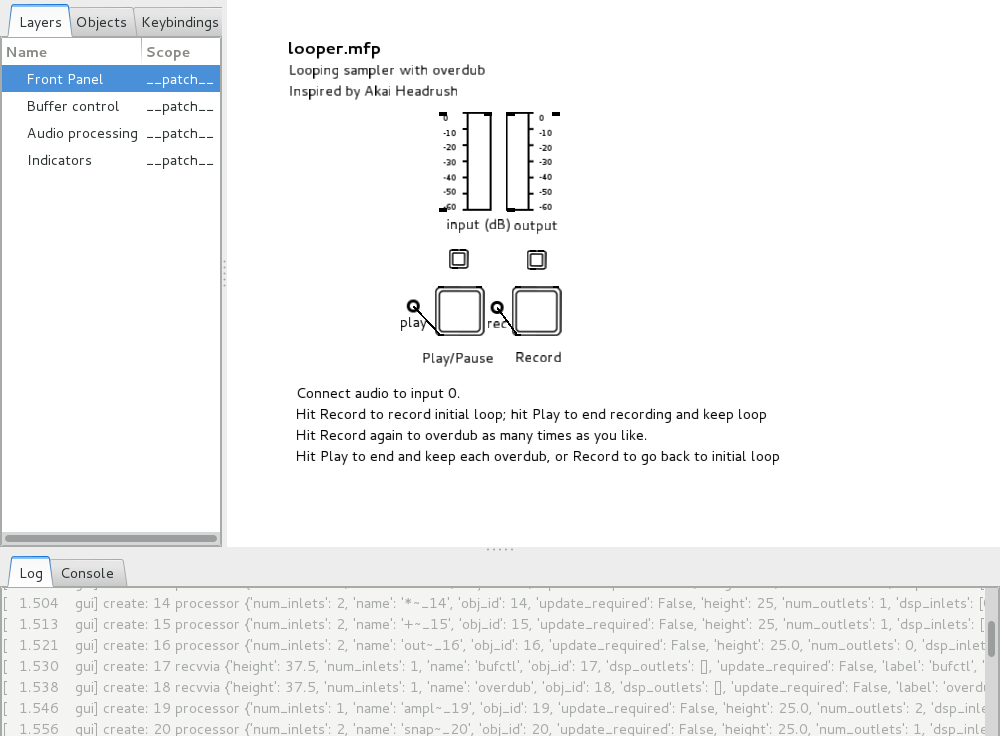
\includegraphics[width=3in]{looper-front.png}
    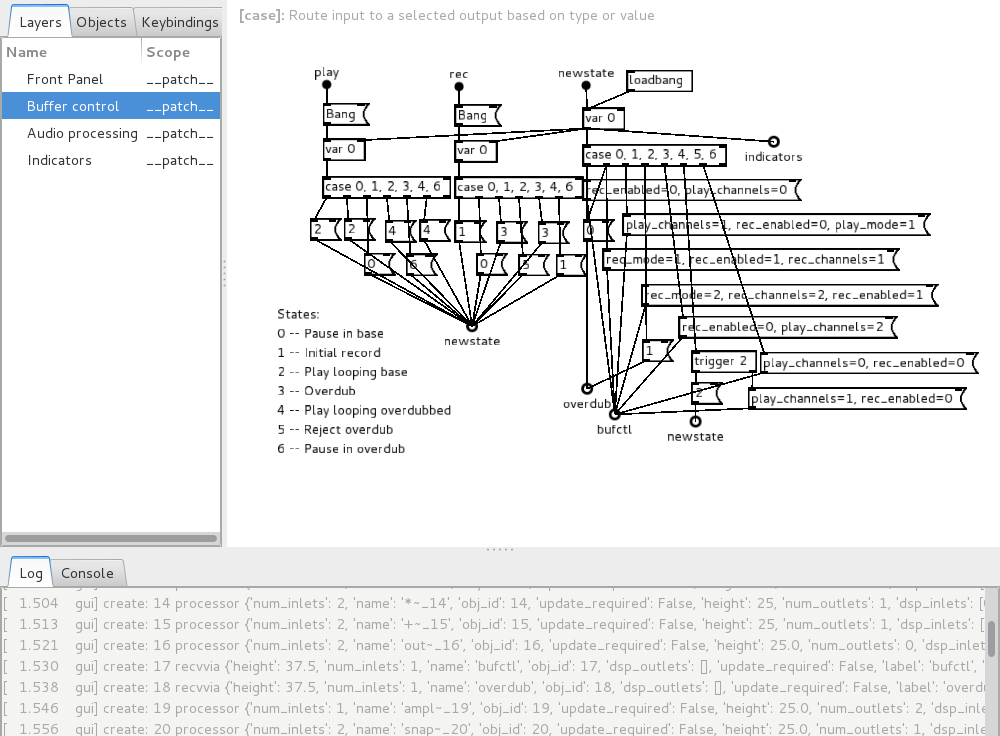
\includegraphics[width=3in]{looper-buffer.png}
    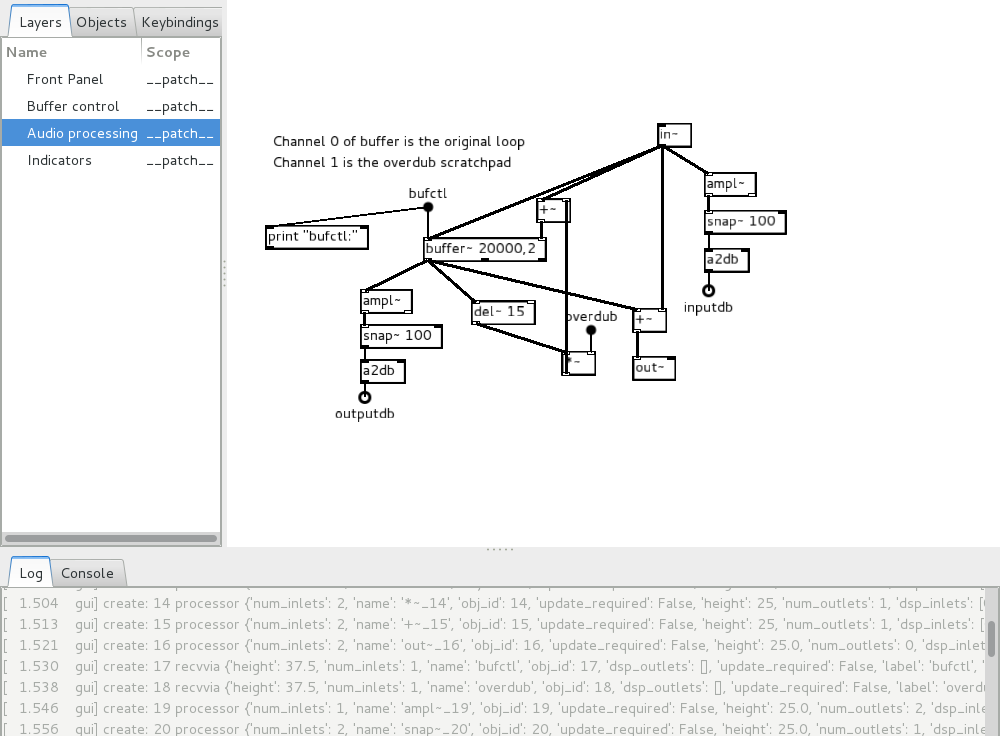
\includegraphics[width=3in]{looper-audio.png}
    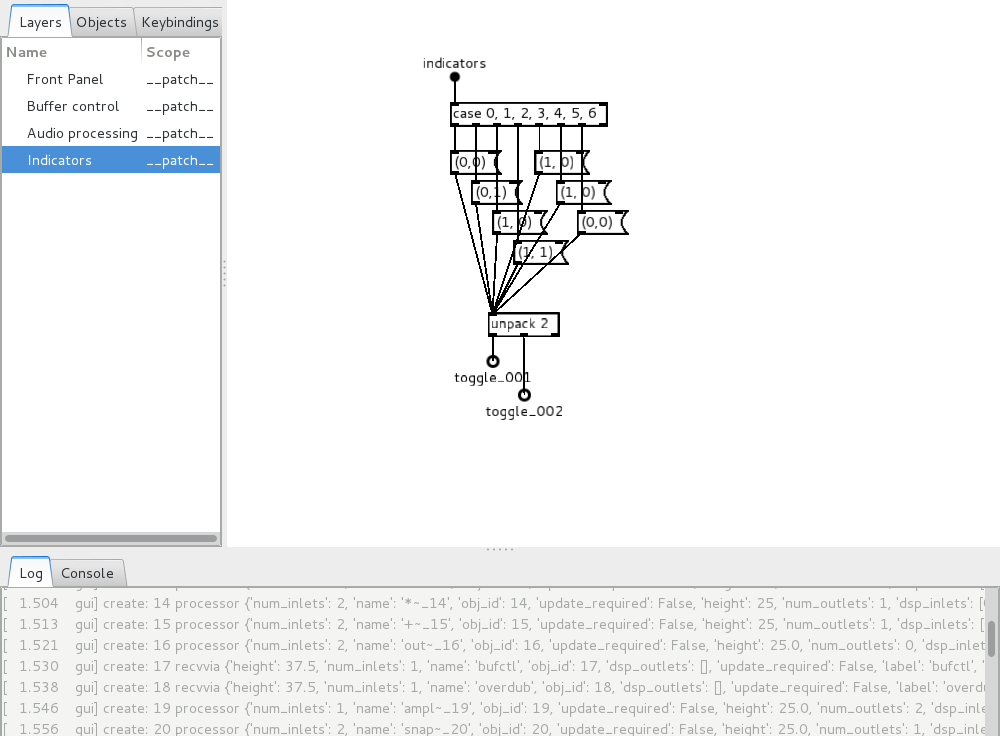
\includegraphics[width=3in]{looper-indicators.png}
    \caption{Looping sampler (\texttt{doc/looper.mfp})}
\end{figure}

This patch demonstrates how layers enable program decomposition in a 
way similar to Pure Data's subpatches.  Each layer contains a block of
functionality, with send/receive vias showing names for inputs and outputs
of the block.  The organization is not as structured as Pure Data's
subpatches, but has the advantage of being clearly a different mechanism
from patch reuse (Pure Data ``abstraction'').

The Python-familiar will note that the contents of many of the message
boxes in the Buffer Control layer (those which are a series of
comma-separated \texttt{key=value} assignments) are not exactly valid
Python code.  This is MFP-specific syntactic sugar for the Python
expression \texttt{dict(key1=value1, key2=value2)} to create a dictionary
object.

\subsection{Control domain}

The control domain is the backbone of MFP's processing, and the control
node is the master and controller of the MFP application.   

The control node hosts zero or more patches, where each patch is an
instance of the \texttt{Patch} class.  Each \texttt{Patch} consists of a
connected graph of processors (instances of the \texttt{Processor} class).
A \texttt{Processor} instance has one or more inlets and zero or more
outlets.  Each inlet may be connected to zero or more outlets of other
processors, and each outlet to zero or more inlets of other processors.
Communication between processors consists of sending a message from an
outlet of one processor to an inlet of another.  The distinguishing feature
of control domain communication is that it happens in discrete chunks
called \emph{messages}. 

Messages sent between processors in the control domain are ordinary Python
objects of any type: numbers, strings, lists, dicts, functions, or other
class instances.  This is significantly different from Pure Data and other
patching languages, which define a limited set of ``atom'' types that can be
used within the patch.   

In many cases it is useful to think of a message processor as a function or
method, where the arity is determined by the number of inlets.  This model
is supported by MFP's default marshaling policy, which buffers inputs to
all inlets until a message is received on a ``hot'' inlet.  Pure Data also
takes this approach.  By  default, only the leftmost inlet (inlet 0) is
``hot'', but that behavior may be changed by a particular
\texttt{Processor} subclass.  The processor's trigger method is then called
to perform message processing.  Functions of null arity are triggered by
any input on their inlet (by convention, the special value \texttt{Bang}).

\subsubsection{Method calls and dispatching}

In other cases it is useful to think of a processor as an object with
methods of its own.  For example, a number box might have an API to control
the number of decimal digits to display.  In interactive usage,
configuration of this property might be accomplished by a dialog or key
sequence, but the underlying mechanism is going to call a
\texttt{configure} method somewhere down the line.  In the spirit of
exposing Python where possible, we allow patches to directly call methods
on the objects that make up the patch.  

The control domain structure of MFP matches fairly neatly with a
\emph{message passing} metaphor for method calls.  A method is called on a
control-domain object by sending it a message representing the method call.
In MFP, the message is an instance of \texttt{MethodCall}.  This object
captures the name and any arguments of the method call (other than the
object to call the method on, which is always the recipient of the
\texttt{MethodCall} message). 

MFP provides classes and syntax to support this style of usage by allowing
for concise and flexible creation of \texttt{MethodCall} objects.  The
example in Figure 3 shows a patch fragment that uses
\texttt{@conf(digits=3)} as syntactic sugar for \texttt{MethodCall("conf",
digits=3)}.  When this message is received by the number box, the method
\texttt{conf} is called, with the keyword argument \texttt{digits} having
the value of 3.  The \texttt{conf} method is supported by all
\texttt{Processor} instances as a way to directly set GUI display
parameters.  

Note that this activity is represented by objects in the graphical domain
(mostly \texttt{PatchElement} subclasses) but the Python evaluation and
message passing all takes place in the control domain. 

\begin{figure}
    \centering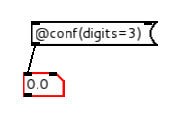
\includegraphics[width=2in]{enum_control.png}
    \caption{Sending a method-call object to change displayed digits 
    (\texttt{doc/enum\_control.mfp})}
\end{figure}

User patches can dispatch their own method calls using the
\texttt{[dispatch]} builtin.  This processor outputs any method call
objects sent to the patch as a \texttt{(name, MethodCall)} tuple suitable
for input into the \texttt{[route]} processor.  The companion
\texttt{[baseclass]} processor handles method resolution for methods
implemented by the base class.  Figure 4 shows a patch fragment handling
dispatch of methods \texttt{m1}, \texttt{m2}, and \texttt{m3}, while
passing all others back to the \texttt{Patch} class for resolution as
methods of the Python \texttt{Patch} class or its base class
\texttt{Processor}.   

\begin{figure}
    \centering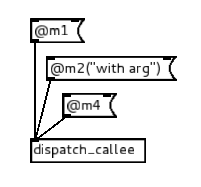
\includegraphics[width=2in]{dispatch_caller.png}
    \centering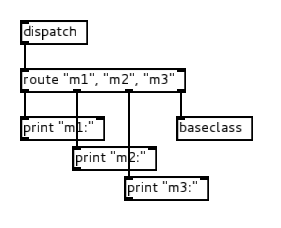
\includegraphics[width=2in]{dispatch_callee.png}
    \caption{Custom method dispatch
    (\texttt{doc/dispatch\_caller.mfp}, \texttt{doc/dispatch\_callee.mfp})}
\end{figure}

\subsubsection{Names and scoping}

At first glance, names may not seem to be that important in a patching
language.  Patch connections directly designate the caller and callee
objects without need for names.  In reality, larger patches need to hide
some connections for readability and structure.  Pure Data provides the
\texttt{[s name]} and \texttt{[r name]} pair (send/receive), which create a
``virtual patch cable'', as well as some special message-box syntax to send
messages directly to an \texttt{[r]}.  MFP uses send/receive via pairs for
the same purpose.  In both cases, names are required to connect sender to
receiver.

MFP gives each \texttt{Patch} a lexical scope, and allows each layer of the
patch to either use the patch scope or to specify a different one.
Separate scopes can make it possible to hygienically copy a layer or a
group of layers without name collisions.  For example, a synthesizer patch
could use hygienic layer duplication to create a dynamic number of
polyphonic voices, if a single voice was built in a layer or set of layers
sharing a scope distinct from the patch scope. 

As a consequence, there is no need to ``mangle'' names to make them unique
to a patch instance in MFP.  Names are automatically scoped within the
patch instance where they are created.  This contrasts with Pure Data,
where names are global by default; names intended to be local use the magic
variable \texttt{\$0}, which expands to a unique-per-patch symbol, as part
of the variable name.  For instance, the name \texttt{foo} would be global,
and a message sent to \texttt{foo} from any open patch will go to all
recipients of \texttt{foo} messages.  \texttt{\$0-foo} would be local to
the patch containing it. 

\subsection{Signal domain}

The signal domain component of MFP is primarily implemented in a C library
containing the Python extension \texttt{mfpdsp}.  MFP uses the JACK Audio
Connection Kit (JACK) \cite{JACK} to interface with the system audio
hardware and other audio applications. 

As in the control domain, processing is implemented in a connected graph of
processing nodes.  However, communication between nodes is a block-based
stream of sample data rather than a sequence of messages. For simplicity,
the processing block size used is always the JACK block size, but this will
likely change in future releases.  

A patch element which performs signal processing activity will have both a
control domain representation (an instance of a \texttt{Processor} class)
and a signal domain representation (a C-allocated instance of
\texttt{struct mfp\_proc}).  The identity between the two is maintained
using an integer \texttt{obj\_id} which is shared. 

JACK does the hard work in the signal layer, and there are only a few
built-in DSP operations (about 20 in all) which, frankly, are not that
interesting: arithmetic, comparisons, simple oscillators/noise,
delay/buffering, simple filters, envelope follower.  It is expected that
LADSPA (and, later: LV2, etc) plugins (\cite{LADSPA}, \cite{LV2}) will
provide the more sophisticated DSP processing tools. 

The graph topology of the signal processing network imposes some ordering
on execution of the node algorithms.  A particular node is only ready to
process when all its inputs have been computed.  To manage this, a simple
scheduling step is performed whenever nodes are added or removed.  Units
that are marked as \emph{generators} (their output in a particular
processing cycle is not dependent on their input during that cycle) are
always ready to process, nodes directly connected to them may be processed
next, and so on.  It is possible for cycles in the connectivity graph to
make a network that cannot be scheduled.  In this case, a delay of at least
one processing block must be added to break the cycle. 

Communication within the signal layer is driven by the JACK callback thread
and is decoupled from the message domain.  Interaction between message and
signal occurs at block boundaries and consists of parameter get/set and
simple messages from the signal back to the message layer.  This allows the
real-time component of the system to operate without a dependency on the
timeliness of processing in the message domain.

\subsection{Graphical domain}

The graphical UI borrows its appearance heavily from Pure Data.  Each
processor is represented by a visual element, with connections represented
by lines.  Most processors have simple flow-chart style representations, 
with distinctive shapes providing cues as to their function. 

Control of the UI is largely keyboard-driven.  The modal input system is
patterned after text editor controls, stacking modes based on the current
context.  Authoring and editing of a patch can be accomplished without
using the mouse or touchpad at all, though a combination of pointing and
typing is more efficient.

The UI is implemented using the Clutter (\cite{Clutter}) and Gtk+ toolkits.
Figure 5 shows samples of each visual type of element, though one
representation (such as the button) can have several distinct identities
depending on parameters (clickable or display only, momentary or latching,
etc).  The functional element types are: 

\begin{figure}
    \centering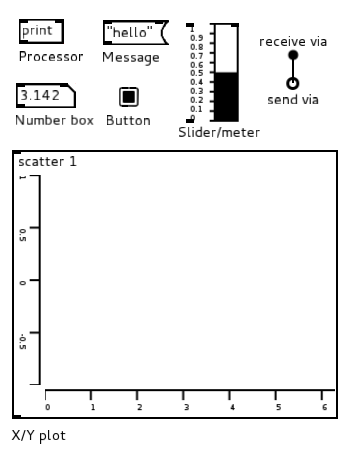
\includegraphics[width=3in]{gui_elements.png}
    \caption{Graphical patch element types (\texttt{doc/gui\_elements.mfp})}
\end{figure}


\textbf{Processor box:} The most common element, a plain box containing the name
and initialization arguments of the processor.  Arguments are interpreted
by the Python evaluator at creation time.

\textbf{Message box:} Interactive element emitting a message when clicked.
The message is displayed in the element and is interpreted by the Python
evaluator when entered through the GUI.

\textbf{Text comment:}  Free text display.  Uses Pango 
markup\footnote{An SGML-like syntax, see 
\url{http://www.gtk.org/api/2.6/pango/PangoMarkupFormat.html}} 
to enable a variety of text styles, sizes, fonts, and colors.

\textbf{Slider control/Bar meter display:} Vertical or horizontal
slider/meter with optional scale display.  Displays a solid bar indicating
a value, draggable for slider control 

\textbf{Number box:} A simple box for interactively entering or editing a
number.  Responds to mouse and keyboard actions to increment/decrement the
value, and emits the value as a message when it is changed. 

\textbf{X/Y chart:} Multi-curve scatter/line chart with plot, roll, and
signal-view (oscilloscope) modes.  Can work in the control domain as a
scatter plot or strip chart, or in combination with a shared memory signal
buffer as an oscilloscope-type display.

\textbf{Toggle button/indicator:} Two-state button with visual indicator of
on/off state.  When created as an indicator, it shows the underlying state
but does not respond to clicks.

\textbf{Momentary (``bang'') button:} Emits a \texttt{Bang} object (or other object as
configured) when clicked.  This is similar to a message box, but does not
display the value to be sent. 

\textbf{Send and receive vias:}  Circular pads representing the end points
of an invisible virtual patch cord (\texttt{[s name]} and \texttt{[r name]}
in Pure Data).  The name and appearance are inspired by printed circuit
board vias, which are conductive pathways connecting one layer of a circuit
board to another. 

\section{Extensibility} 

User-created processing modules in the signal and message domains can be
loaded at runtime via several mechanisms:

\textbf{Patch file discovery.}  When a reference  to an unknown processor
type is made, the search path is crawled to find a patch file (*.mfp) with
a matching  name.  User patches are equivalent to builtins, except for the
additional overhead of network iteration.  

\textbf{Processor subclassing.}  User code loaded at startup or patch load
time can create new Processor subclasses which can be referenced in
patches.

\textbf{User-specified function wrapping.}  A utility API is provided to
wrap arbitrary Python functions or methods as MFP processors.  Code in user
rcfile or other startup file can create simple or complex processor types
using these tools.

\textbf{Automatic Python callable wrapping.}  An attempt to create a
Processor will succeed if any Python function with the specified name is
known to the MFP evaluator at runtime.  The matching function will be
automatically wrapped in a simple Processor subclass that uses
introspection to discover the arity of the provided function.  

\textbf{Compiled DSP processor definitions.}  Dynamically linked libraries
containing DSP type definitions can be loaded at runtime via
\texttt{dlopen}.  A simple C-language processor type definition API makes
creation of new unit types straightforward.  

\textbf{Plugin hosting.}  LADSPA plugins can be hosted and controlled via
the \texttt{[plugin\textasciitilde]} builtin.

\section{Interoperability} 

MFP implements interfaces to other software via open standards:

\textbf{JACK:}  MFP is a standalone JACK application.  The number of input
and output ports is specified at app startup time.   Support for JACK MIDI,
transport, and timecode is planned. 

\textbf{Open Sound Control (OSC):}  Every MFP object  in the control domain
has an OSC address and can receive messages in numeric or Python expression
form.  Every \texttt{Processor} supports OSC controller learning via the
\texttt{@osc\_learn} method. OSC message send and additional routing for
incoming messages are provided through builtin processors
\texttt{[osc\_in]} and \texttt{[osc\_out]}.

\textbf{MIDI:}  The ALSA sequencer API is used to provide MIDI I/O.  MIDI
data is processed in the message domain, and is routed in and out via the
\texttt{[midi\_in]} and \texttt{[midi\_out]} builtins.  Chasing and
generating MIDI timecode is planned. 

\textbf{LADSPA:}  A builtin DSP type hosts LADSPA plugins.  LADSPA plugin 
meta-information is used to add input and output ports for all plugin 
parameters at run time. An LV2 host is planned.  

\section{Implementation status}  

As of the submission of this paper (Feb 2013) MFP is under heavy
development leading up to an initial public release.  The functionality
described in this document is implemented and exercised by demonstration
patches provided in the source code repository. 

Much of the development process has been exploratory in nature, so the
feature set as a whole is a bit spotty.  Significant features are missing
or incomplete, including the ability to have more than one patch open for
editing, exported patch UIs (``graph-on-parent''), hosting LV2 and other
types of plugins, support for session APIs, online help and other
documentation, undo/redo, menu control of most functions, and saved
configurations (presets) in patches. 

\section{Getting MFP}

Source code and issue tracking for MFP are on GitHub:

\begin{quote}
\texttt{https://www.github.com/bgribble/mfp}
\end{quote}

The project is licensed under the GNU General Public License (GPL) version
2.   Your interest and participation is invited and welcomed.


%Text of the subsection with citations such as 
%\cite{Spa72}, \cite{Kay86} and \longcite{MosWal64}.
%
%\begin{table}[h]
% \begin{center}
%\begin{tabular}{|l|l|}
%
%      \hline
%      Software & Features\\
%      \hline\hline
%      AA & Harddisk-Recording\\
%      BB & MIDI Sequencing\\
%      CC & Score Notation\\
%      \hline
%
%\end{tabular}
%\caption{Example}\label{table1}
% \end{center}
%\end{table}
%

\bibliographystyle{acl}
%\bibliographystyle{plainnat}
\bibliography{lac2013}

\end{document}
